\documentclass{article}
\usepackage{graphicx}
\usepackage[section]{placeins}
\usepackage{xcolor}
\usepackage{hyperref}
\hypersetup{
    colorlinks=true,
    linkcolor=blue,
    filecolor=magenta,      
    urlcolor=cyan,
}
\usepackage[utf8]{inputenc}
\usepackage{listings} % nice code layout
\lstset{language = Verilog}
\lstset{language = C++}
\graphicspath{ {./img/} }
\usepackage[a4paper, margin=1.25in]{geometry}


\author{Justin Bui}
\title{Microblaze Implementation of a 7 Segment Display Controller}

\begin{document}

\maketitle
\newpage

\tableofcontents
\newpage

\section{Introduction}
This document outlines the design and implementation for the 7 Segment Display system. This project makes use of the Digilent NEXYS 4 Artix-7 FPGA development board to implement a Microblaze based 7 Segment display system. The document below includes the functional description, code portions, and implementation of the project. 


\section{Project Description}
The 7 Segment display control system is designed to control the 8 displays present on the Nexys 4 development board. Based on the 32bit Microblaze softcore, this project provides the HDL and drivers necessary to make use of the 7 Segment displays in which ever manner use deems fit. Each display module can be configured individually (that is, independently from one another), allowing for extended flexibility. 

\section{Core Code}
The core functionality of the 7 Segment Display controller is derived from two System Verilog files, the disp\_hex\_mux.sv and bui\_disp\_core.sv. The primary module comprises all 8 of the display modules, as well as control for the decimal points. The module is passed into the display core, which provides the wrapping circuit to connect the display module to the CPU. The base module code is shown below.

\begin{lstlisting}[language = Verilog]

module disp_hex_mux(
        input logic clk, reset,         // Clock and reset Signals
        input logic [3:0] val7, val6, val5, val4, val3, val2, val1, val0,    
        input logic [7:0] dp_in,        // decimal point signals
        output logic [7:0] an,          // Segment Enable Bits
        output logic [7:0] sseg         // 7 segment display output
    );
    
    // internal signals
    localparam N = 18;  // set LED refresh rate to ~ 800Hz
    logic [N-1:0] q_reg;                // Current State
    logic [N-1:0] q_next;               // Next State
    logic [3:0] val;                    // Digit Value
    logic dp;                           // decimal 
    
    // Counter
    always_ff @(posedge clk, posedge reset)
        if(reset)
            q_reg <= 0;
        else
            q_reg <= q_next;
        
    assign q_next = q_reg + 1;
    // Multiplexing For Display    
    always_comb
        case(q_reg[N-1:N-3])
            3'b000:
                begin
                    an = 8'b11111110;
                    val = val0;
                    dp = dp_in[0];
                end
            3'b001:
                begin
                    an = 8'b11111101;
                    val = val1;
                    dp = dp_in[1];
                end
            3'b010:
                begin
                    an = 8'b11111011;
                    val = val2;
                    dp = dp_in[2];
                end
            3'b011:
                begin
                    an = 8'b11110111;
                    val = val3;
                    dp = dp_in[3];
                end
            3'b100:
                begin
                    an = 8'b11101111;
                    val = val4;
                    dp = dp_in[4];
                end
            3'b101:
                begin
                    an = 8'b11011111;
                    val = val5;
                    dp = dp_in[5];
                end
            3'b110:
                begin
                    an = 8'b10111111;
                    val = val6;
                    dp = dp_in[6];
                end
            default:
                begin
                    an = 8'b01111111;
                    val = val7;
                    dp = dp_in[7];
                end
                    
         endcase
      // Individual 7-Segment Display Values 
      always_comb
            begin
                case(val)
                    4'h0: sseg[6:0]=7'b1000000; // '0'
                    4'h1: sseg[6:0]=7'b1111001; // '1'
                    4'h2: sseg[6:0]=7'b0100100; // '2'
                    4'h3: sseg[6:0]=7'b0110000; // '3'
                    4'h4: sseg[6:0]=7'b0011001; // '4'
                    4'h5: sseg[6:0]=7'b0010010; // '5'
                    4'h6: sseg[6:0]=7'b0000010; // '6'
                    4'h7: sseg[6:0]=7'b1111000; // '7'
                    4'h8: sseg[6:0]=7'b0000000; // '8'
                    4'h9: sseg[6:0]=7'b0010000; // '9'
                    4'ha: sseg[6:0]=7'b0001000; // 'A' 
                    4'hb: sseg[6:0]=7'b0000011; // 'B' 
                    4'hc: sseg[6:0]=7'b1000110; // 'C' 
                    4'hd: sseg[6:0]=7'b0100001; // 'D' 
                    4'he: sseg[6:0]=7'b0000110; // 'E' 
                    default: sseg[6:0]=7'b0001110; // Default 'F'
                endcase
                sseg[7] = dp;
            end
endmodule

\end{lstlisting}

The core and wrapping circuit is shown display. I have written the core to make use of three data registers, 1 register for the left 4 display units, a second register for the right 4 display units, and a third register to track the decimal points. 

\begin{lstlisting}[language = Verilog]
module bui_disp_core(
    // Logic Inputs
    input  logic clk,
    input  logic reset,
    // Slot Inputs
    input  logic cs,
    input  logic read,
    input  logic write,
    input  logic [4:0] addr,
    input  logic [31:0] wr_data,
    // Slot Outputs
    output logic [31:0] rd_data,
    // 7 Segment Outputs
    output logic [7:0] an,
    output logic [7:0] sseg
    );
   
   // Internal Registers
   logic [31:0] data_reg2, data_reg1, data_reg0;
   logic write_en, write_d2, write_d1, write_d0;
   // Create Display Unit
   disp_hex_mux disp_unit (.clk(clk), .reset(reset), .val7(data_reg1[31:24]), 
				.val6(data_reg1[23:16]), .val5(data_reg1[15:8]), 
				.val4(data_reg1[7:0]), .val3(data_reg0[31:24]),
                            	.val2(data_reg0[23:16]), .val1(data_reg0[15:8]),
				.val0(data_reg0[7:0]),
                            .dp_in(data_reg2[7:0]), .an(an), .sseg(sseg));
   // always FF setup
   always_ff @(posedge clk, posedge reset)
        if(reset)
            begin
                data_reg2 <= 0;
                data_reg1 <= 0;
                data_reg0 <= 0;
            end
        else
            begin
                if(write_d0)
                    data_reg0 = wr_data;
                if(write_d1)
                    data_reg1 = wr_data;
                if(write_d2)
                    data_reg2 = wr_data;
            end
    // Write Register Controls
    assign write_d0 = write & cs & ~addr[0] & ~addr[1]; // Low 4 disp
    assign write_d1 = write & cs & addr[0] & ~addr[1];  // High 4 disp
    assign write_d2 = write & cs & addr[1];             // Decimal Point     
    // Read Data Register Unused
    assign rd_data = 0;   
endmodule
\end{lstlisting}

\section{Microblaze Implementation}
Now that the core and wrapping circuits have been built up, it must be integrated into the Microblaze. This is accomplished by implementing the wrapper described above into the mmio\_sys\_vanilla.sv file originally provided by Pong Chu. As Chu has already provided a slot for the his implementation of the 7 Segment Display, I have opted to make use of the same slot.

\begin{lstlisting}[language=Verilog]
 // slot 8: 7 Segment Display
    bui_disp_core sseg_slot8
    (.clk(clk),
     .reset(reset),
     .cs(cs_array[`S8_SSEG]),
     .read(mem_rd_array[`S8_SSEG]),
     .write(mem_wr_array[`S8_SSEG]),
     .addr(reg_addr_array[`S8_SSEG]),
     .rd_data(rd_data_array[`S8_SSEG]),
     .wr_data(wr_data_array[`S8_SSEG]),
     .sseg(sseg),
     .an(an)
     );
     
\end{lstlisting}

\newpage

\section{Software Implementation}
The software impelmentation for this project makes use of some of Pong Chu's core files (such as his timer functions), as well as a small demo function. This demo function uses 6 of the 8 displays to show a 1 second counter in hexidecimal format (as opposed to traditional binary). The counter is set to run long enough to demonstrate several of the display modules, as well as using the decimal point. 

	\begin{figure}[h!]
		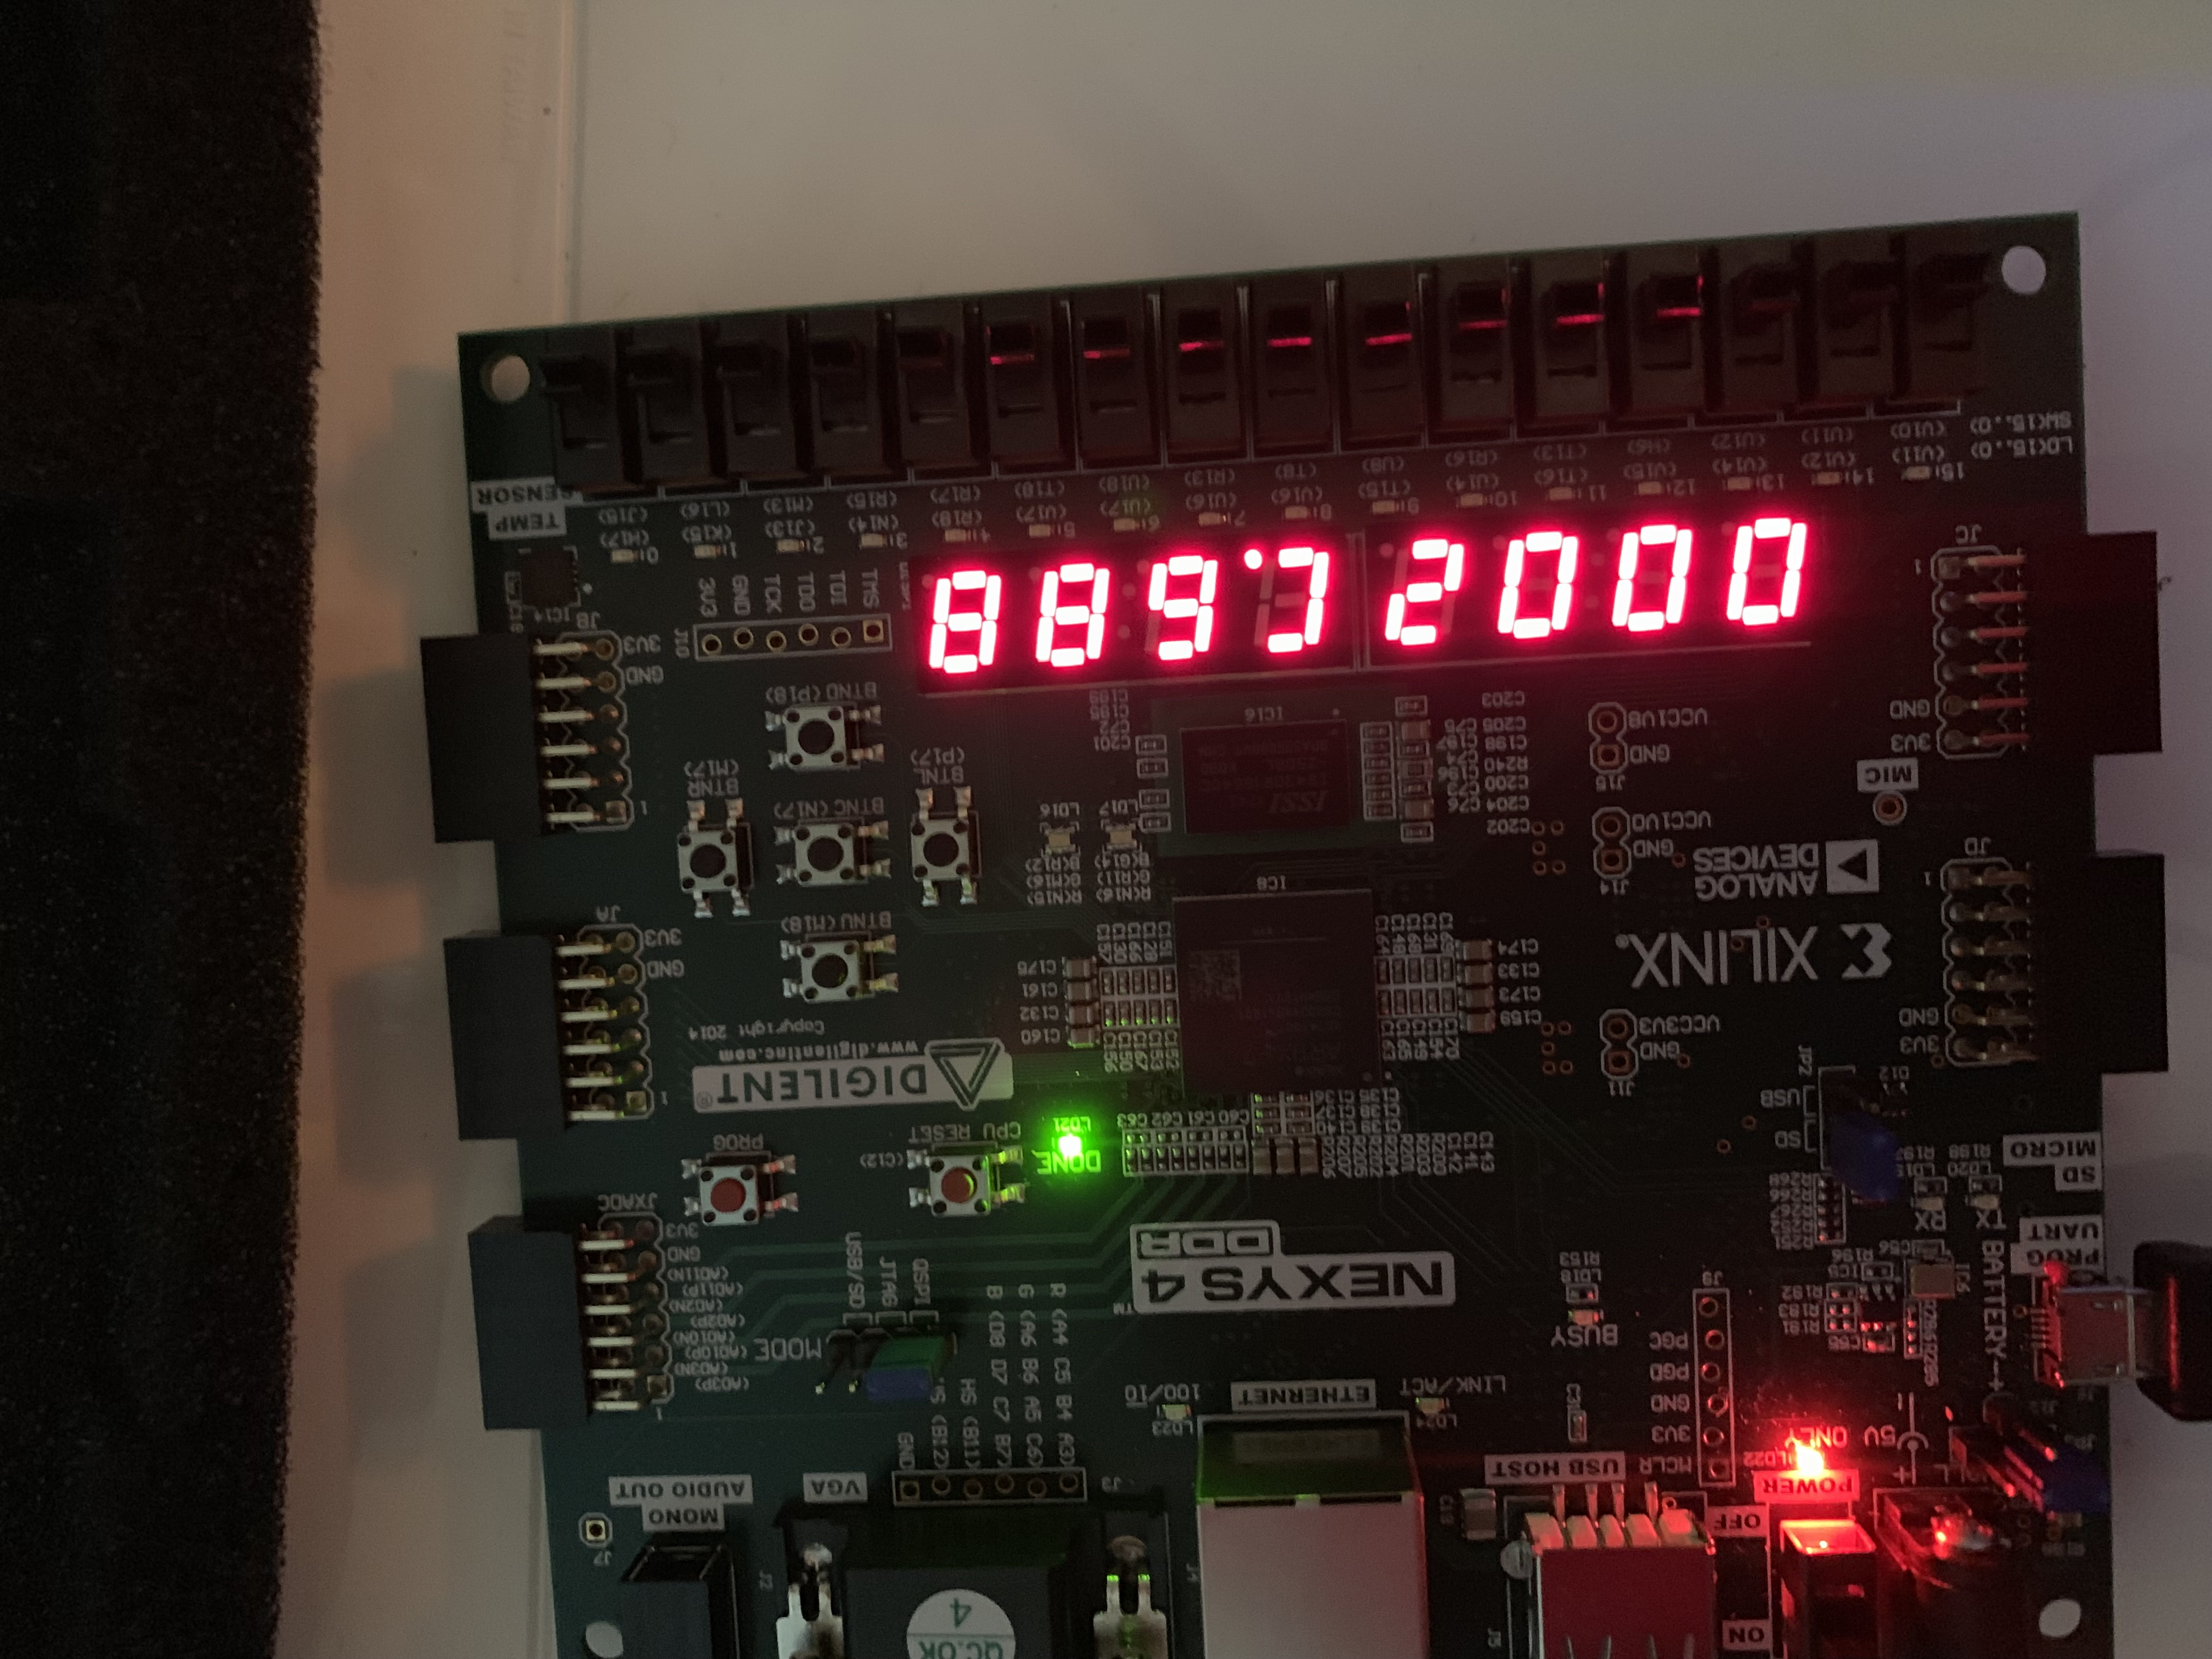
\includegraphics[width=.9\linewidth]{d1.JPG}
		\caption{7 Segment Display Demo}
	\end{figure}
Class Definition Code:
\begin{lstlisting}[language=C=++]
class ssegCore {
public:
   /**
    * Register map
    */
   enum {
      DATA_LOW_REG = 0, 	// 32-bit data for right 4 digits
      DATA_HIGH_REG = 1, 	// 32-bit data for left 4 digits
	  DATA_DP_REG = 2		// 32-bit data, LSB for DP
   };
private:
   /* variable to keep track of current status */
   uint32_t base_addr;
   uint8_t ptn_buf[8];    // led pattern buffer
   uint8_t dp;            // decimal point
   /* methods */
   void write_disp();      // write patterns to reg
}
;
\end{lstlisting}

Test Function Code:
\begin{lstlisting}[language=C++]
void sseg_check(ssegCore *sseg_p) {
   int h,i,j,k,l,m;
   uint8_t dp;

   //turn off led
   for (i = 0; i < 8; i++) {
      sseg_p->write_1ptn(0xff, i);
   }
   //turn off all decimal points
   sseg_p->set_dp(0x00);

   // display 0x0 to 0xf in 4 epochs
   // upper 4  digits mirror the lower 4
   for (h = 0; h < 15; h++) {
      for (i = 0; i < 16; i++) {
	  for(j = 0; j <16; j++)
	  {
		  if(j>0)
			  sseg_p->set_dp(0x08);		// seconds decimal point
		  for(k=0; k<16; k++){
			  for(l=0; l<16; l++){
				  for(m=0; m<16; m++){
				  sseg_p->write_1ptn(sseg_p->hexToDisp(m), 0);
				  sseg_p->write_1ptn(sseg_p->hexToDisp(l), 1);
				  sseg_p->write_1ptn(sseg_p->hexToDisp(k), 2);
				  sseg_p->write_1ptn(sseg_p->hexToDisp(j), 3);
				  sseg_p->write_1ptn(sseg_p->hexToDisp(i), 4);
				  sseg_p->write_1ptn(sseg_p->hexToDisp(h), 5);
				  sseg_p->write_1ptn(sseg_p->hexToDisp(0), 6);
				  sseg_p->write_1ptn(sseg_p->hexToDisp(0), 7);
				  sleep_us(244);	// 244us cycles 0-4096, 1s
				  }
			  }
		  }
	  }
  }

}
\end{lstlisting}

\end{document}